% !TeX encoding = UTF-8
% !TeX program = xelatex
\documentclass[12pt, a4paper]{article}
\usepackage{xeCJK} % 须放在\usepackage{}列中足够前的位置
\usepackage{fontspec}
\usepackage{graphicx} % 插入圖片
\usepackage{caption}
\usepackage{enumerate}
\usepackage{setspace}
\usepackage{array} % 製作表格必須的宏包
\usepackage{tabularx} % 自動調整列寬的表格宏包
\usepackage{adjustbox}
\usepackage{geometry} 

% -- Loading the code block package:
\usepackage{listings}
% -- Basic formatting
\usepackage[utf8]{inputenc}
\usepackage[english]{babel}
\usepackage{times}
\usepackage{listings}
\usepackage{xcolor}

\definecolor{codegreen}{rgb}{0,0.6,0}
\definecolor{codegray}{rgb}{0.5,0.5,0.5}
\definecolor{codepurple}{rgb}{0.58,0,0.82}
\definecolor{backcolour}{rgb}{0.95,0.95,0.92}

\lstdefinestyle{mystyle}{
    backgroundcolor=\color{backcolour},   
    commentstyle=\color{codegreen},
    keywordstyle=\color{magenta},
    numberstyle=\tiny\color{codegray},
    stringstyle=\color{codepurple},
    basicstyle=\ttfamily\footnotesize,
    breakatwhitespace=false,         
    breaklines=true,                 
    captionpos=b,                    
    keepspaces=true,                 
    numbers=left,                    
    numbersep=5pt,                  
    showspaces=false,                
    showstringspaces=false,
    showtabs=false,                  
    tabsize=2
}

\lstset{style=mystyle}


\setCJKfamilyfont{heiti}{Heiti TC}
\CJKfamily{heiti}
\setmainfont{Arial}
\setstretch{1.5}


\begin{document}
  \begin{center}
    {\Huge 資料結構實習} \\[2.5cm]
    {\Huge 10/06 作業報告} \\[1.5cm]
    {\Huge 多項式ADT實作} \\ [4.5cm]
    \hspace{.6in}
    \begin{minipage}[t]{.4\linewidth}
      {\Large 班級:資訊二甲}\\[0.5cm]
      {\Large 學號:D1109023}\\[0.5cm]
      {\Large 姓名:楊孟憲}
    \end{minipage}    
  \end{center}

  \newpage

  \begin{samepage}
    \fontsize{18pt}{20pt} \selectfont  
    % 生成目錄
    \tableofcontents
    \normalfont
  \end{samepage}
  
  \newpage


  \section{\fontsize{20pt}{22pt}\selectfont 引言}
  \begin{samepage}
    \fontsize{16pt}{18pt} \selectfont
    今天要使用 struct (結構) 來實作多項式的操作運算。
    \lstinputlisting[language=C++]{../code/template.cpp}
  \end{samepage}

  % 第一個章節

  \section{\fontsize{20pt}{22pt}\selectfont 題目敘述}
  \begin{samepage}
    \fontsize{16pt}{18pt} \selectfont
        題意說明:撰寫一個程式,讀取 B1.txt 以及 B2.txt 多項式內容,並包含以下功能。
        請提供選單的方式,讓使用者能夠對此多項式 ADT 做操作:
        \begin{enumerate}
            \fontsize{14pt}{16pt} \selectfont
            \item 讀入多項式
            \item 印出多項式內容
            \item 多項式相加
            \item 多項式乘上一數值
            \item 印出多項式中最大指數的係數
            \item 新增項式
            \item 刪除多項式中的項
            \item 多項式相乘
        \end{enumerate}
  \end{samepage}
  % 第二個章節

  \section{\fontsize{20pt}{22pt}\selectfont 作法}
  % 第二章節的子章節
  \begin{samepage}
    \fontsize{16pt}{18pt} \selectfont
    因為這個題目需要不斷輸入你所需要的功能 $(1 \sim 8)$,所以使用 while loop 來做最外圍的流程控制,依照不同的輸入來呼叫相對應功能的函式。
    以下介紹代碼中的函式( 程式碼講解在註解裡 )
    \begin{enumerate}
      \item void MyPoly::refresh(const char* filename)
      \lstinputlisting[language=C++]{../code/src/refreash.cpp}
      \item void MyPoly::ShowPoly() 
      \lstinputlisting[language=C++]{../code/src/show.cpp}
      \item mypoly mypoly::add(mypoly poly2)
      \lstinputlisting[language=C++]{../code/src/add.cpp}
      \item void MyPoly::SingleMult(int n)
      \lstinputlisting[language=C++]{../code/src/SingleMulit.cpp}
      \item int MyPoly::Lead_Exp()
      \lstinputlisting[language=C++]{../code/src/LeadExp.cpp}
      \item void MyPoly::Attach(int coef, int expon)
      \lstinputlisting[language=C++]{../code/src/Attach.cpp}
      \item void MyPoly::Remove(int expon)
      \lstinputlisting[language=C++]{../code/src/Remove.cpp}
      \item MyPoly MyPoly::Mult(MyPoly poly2)
      \lstinputlisting[language=C++]{../code/src/Mult.cpp}
    \end{enumerate}
    \normalfont
  \end{samepage}

  \section{\fontsize{20pt}{22pt}\selectfont 執行結果}
  % 第三個章節
      \fontsize{16pt}{18pt} \selectfont
        輸入輸出結果:(每次輸入後都會輸出結果)
        \begin{figure}[ht]
          \centering
          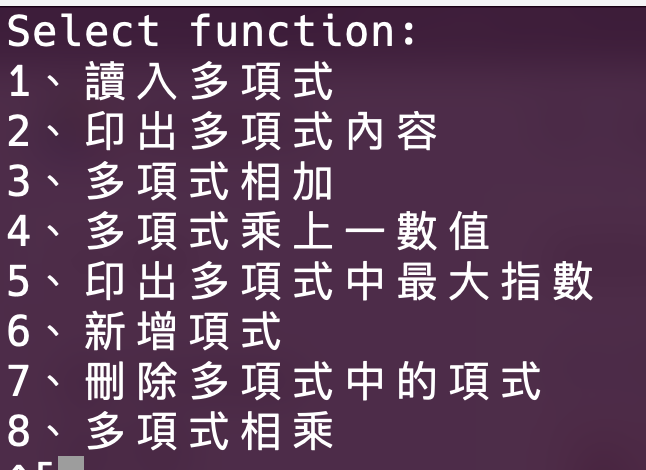
\includegraphics[width=0.6\textwidth]{./image/output.png}
          \caption{選單}
        \end{figure}

        \begin{figure}
          \centering
          
\includegraphics[width=0.6\textwidth]{./image/Show.png}
          \caption{輸入2}
        \end{figure}

        \begin{figure}
          \centering
          
\includegraphics[width=0.6\textwidth]{./image/Add.png}
          \caption{輸入3}
        \end{figure}

        
        \begin{figure}
          \centering
          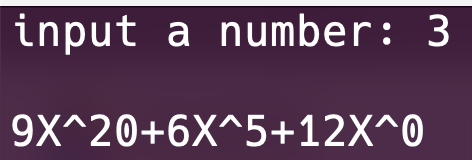
\includegraphics[width=0.6\textwidth]{./image/SingleMult.png}
          \caption{輸入4}
        \end{figure}

        \begin{figure}
          \centering
          
\includegraphics[width=0.6\textwidth]{./image/LeadExp.png}
          \caption{輸入5}
        \end{figure}

        \begin{figure}
          \centering
          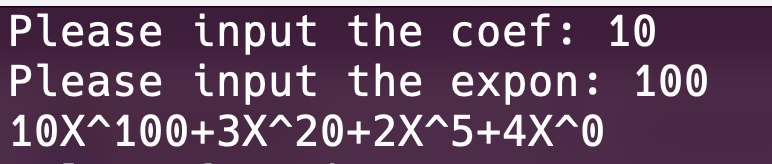
\includegraphics[width=0.6\textwidth]{./image/Attach.png}
          \caption{輸入6}
        \end{figure}
          
        \begin{figure}
          \centering
          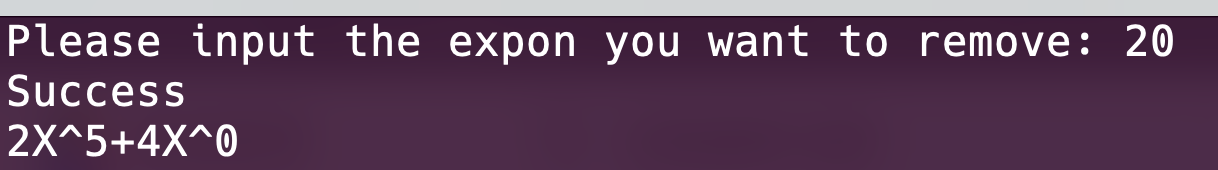
\includegraphics[width=0.6\textwidth]{./image/Remove.png}
          \caption{輸入7}
        \end{figure}

        \begin{figure}
          \centering
          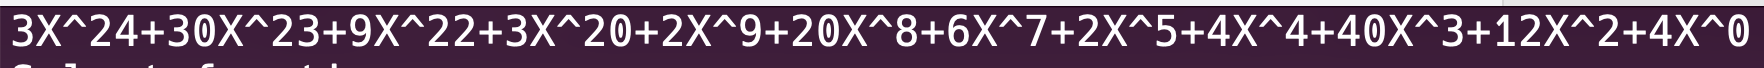
\includegraphics[width=0.6\textwidth]{./image/Mult.png}
          \caption{輸入8}
        \end{figure}


      \normalsize

  \section{\fontsize{20pt}{22pt}\selectfont 心得與討論}
  \begin{samepage}
    \fontsize{16pt}{18pt} \selectfont
      這次的功課實作的部分非常多,在操作不同成員的陣列也要非常小心,陣列索引值需注意現在的變數屬於哪一個而去指定。
      整體來說我覺得可以優化的部分有:陣列可以更改成可以擴充的 vector 等,如此一來,也比較不會操作到不同成員的索引值,而且在做擴充或是刪除的動作也比較簡單。
      以及在 struct 內可以自行定義 operator 排序的方式,這樣就不需每次操作完都排序過。我覺得這次作業能讓我更加了清楚構變數以及函示的使用。
    \normalfont
  \end{samepage}
  % 最後一個章節
\end{document}
